\documentclass[11pt]{article}

\usepackage{fullpage}
\usepackage{xcolor}
\usepackage{graphicx}

\newcommand{\code}[1]{\mbox{\texttt{\textcolor{blue}{#1}}}}

\graphicspath{{./images/}}

\title{ARM Checkpoint... }
\author{Vincent Ho, Kiky Chow, Jasper Liu, Julian Wong}

\begin{document}

\maketitle

\section{Introduction and Group Organisation}

While working on the emulator, the workload was split into several distinct parts which could be done at the same time, reducing the number of merge conflicts on Git. We thus spread the work across several files:

\begin{itemize}
\item \code{computer.c}: Our representation of the computer, including memory and registers
\item \code{fetch.c}: Fetching instructions from memory
\item \code{decode.c}: Distinguishing instruction types
\item \code{execute.c}: Executing instructions by type
\item \code{bit\_implementation.c}: Manipulation on binary values
\end{itemize}

We coordinated our work through regular group meetings on Discord, where we were able to solve coding problems collaboratively along the way. Furthermore, deadlines were also set internally to ensure that everything could be done before submission. It took us about 4 days to finish our individual parts, where we then linked everyone's files together, compiled the program and started the debugging process.

\section{Progress and Reflections}

Overall, our teamwork was harmonious and productive, despite having to work remotely. We effectively split our workload to avoid overlapping and merge conflicts on Git. Constant communication between group members also allowed us to refactor various functions from different parts of the program, thus deleting redundant parts of code. We have since made ourselves more familiar with Git and developed skills to work in a team environment as programmers. We are thus confident in keeping up the strong collaboration to finish the rest of our project.

\section{Structure of the ``Computer''}

Our \code{Computer} struct contains two arrays – the memory and the registers, as well as various privately used registers and flags in order to provide space for data handover between the fetch, decode and execute stages. These include the instruction register (\code{reg\_fetch}), the decoded instruction (\code{reg\_decode}) along with its type (\code{reg\_decode\_type}), the branching flag (\code{flag\_branch}, to indicate that a branch is in progress in the pipeline) and the halt flag (\code{flag\_halt}). Finally, the struct also contains two delay values – \code{delay\_decode} and \code{delay\_execute}, which store the number of loops a stage should wait for before it can start. For example, when the pipeline is empty, the execute stage should not commence until two loops after the fetch stage has started.

\section{Structure of the Emulator}

Every cycle begins with \code{execute}, after which \code{decode} follows, and lastly \code{fetch}. This is to simulate the three stages being run simultaneously. Notice how \code{execute} depends on the output of \code{decode}, which itself depends on \code{fetch}. By ``reversing'' the conventional order, we can ensure that \code{fetch} is one cycle ahead of \code{decode} and two ahead of \code{execute} – the side effects of the pipeline.\\

\begin{figure}[h]
\centering
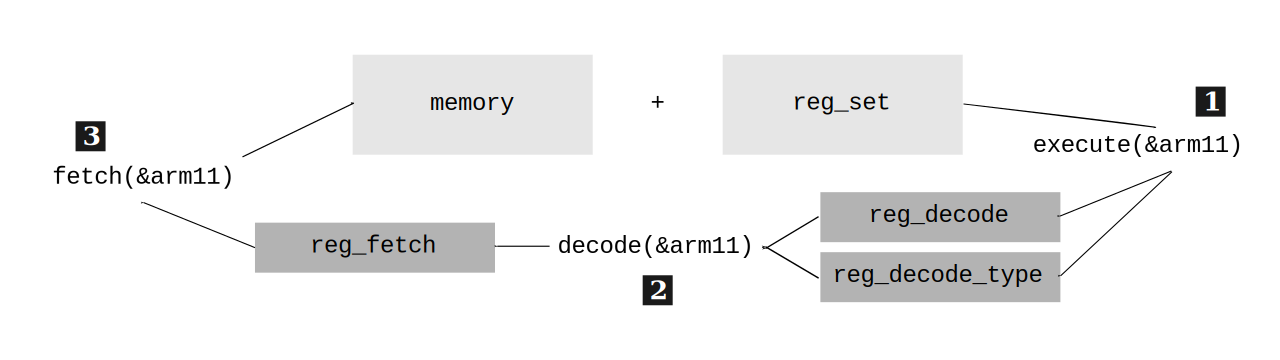
\includegraphics[width=\linewidth]{emulator_flow}
\caption{An illustration of the emulator's three stage pipeline}
\label{fig:emulator_flow}
\end{figure}

To improve the code's readability, we have factored and grouped the sub-functions of \code{execute.c} by instruction type, e.g. \code{single\_data\_transfer(...)}, \code{branch(...)} etc., as well as functions that would be called multiple times, such as \code{operand2\_is\_reg(...)} and \code{rotate\_right(...)}. We have also created multiple enums to store the corresponding values to certain string labels, e.g. the opcode value of a given mnemonic. We would easily need to reuse these features functionally when developing the assembler in Part II. For instance, it would need to be able to correctly generate a binary value when scanning through a mnemonic string.

\section{Difficulties During Development}

With regards to executing instructions, single data transfer instructions have four flags, which make it harder to execute accurately while reducing the duplication of code, especially when differentiating between pre-indexing and post-indexing. Separating the address may also become a challenge when building the assembler later on. Implementing the branch instruction was also a challenge, since it required us to design the aforementioned delay and flag mechanism in order to accommodate for the pipeline's side effects.\\

However, the main problem was not the coding but rather agreeing on an implementation for the emulator, debating on what the most efficient ways were. We will thus utilise this experience and try to hold discussions earlier to allow extra time for planning, and ensure that everyone’s ideas are included in some way.

\end{document}
